% Created 2018-02-05 Mon 21:10
\documentclass[11pt]{article}
\usepackage[utf8]{inputenc}
\usepackage[T1]{fontenc}
\usepackage{fixltx2e}
\usepackage{graphicx}
\usepackage{longtable}
\usepackage{float}
\usepackage{wrapfig}
\usepackage{rotating}
\usepackage[normalem]{ulem}
\usepackage{amsmath}
\usepackage{textcomp}
\usepackage{marvosym}
\usepackage{wasysym}
\usepackage{amssymb}
\usepackage{hyperref}
\tolerance=1000
\date{\today}
\title{WorldCiv}
\hypersetup{
  pdfkeywords={},
  pdfsubject={},
  pdfcreator={Emacs 25.3.1 (Org mode 8.2.10)}}
\begin{document}

\maketitle
\tableofcontents

\section{History 1310 - Science and Technology in World Civilization}
\label{sec-1}

Date: \textit{<2019-01-18 Thu>} Lecturer: Driggers

\subsection{Questions? :email: edriggers@tntech.edu \textbf{Office Hours}:}
\label{sec-1-1}
T-Th: 4:30-6
What are office hours for? 
\begin{itemize}
\item Problems reading and retaining information from lecture or textbook.

\item Questions about grades, performance, participation, attendance, Etc

\item Go over a test or paper

\item Recommendations about improvement
\end{itemize}

\section{Lecture 1 - What is the meaning of Science?}
\label{sec-2}

\begin{itemize}
\item Whare is the use of science?

\item Are there ways that science can be improperly?

\item Is science value free?

\item How do non-epistimic
\end{itemize}

values figure into scientific investigations? 

\begin{itemize}
\item What are the role of

\item contextual values in science?

\item Whose values will impact scientific work?
\end{itemize}

\subsection{What do I mean by Values???}
\label{sec-2-1}

\begin{itemize}
\item Epistimic-Traditionally means values in the internal processes of science? like measuremenquantification, ?Testable?

\item Non-Epistimic-Means those not in the internal process, often effecting the conceptualization of questions and interpretation of ?data,? things like experiences, psychological worries, political values, ideas about race, gender \&c.

\item Objectivity is a changing standard throughout history!
\end{itemize}


\subsection{Traditional Conception of Scientific Investigation}
\label{sec-2-2}
\begin{itemize}
\item Scientists:

\begin{itemize}
\item Observe phenomena, Measure it, and Understand and make products; control phenomena; offer recommendations
\end{itemize}

\item Who are scientists?

\item What is deemed phenomena?

\item What counts as proper measurement?

\item Why are conclusions drawn, verified, and communicated to prfessionals and the public(s)?

\item Is science objective? 

\begin{itemize}
\item What questions are we as society comfortable with asking?

\item What is the role of ethics in scientific investigations?
\end{itemize}
\end{itemize}

\subsubsection{Nazi Medical Experimentation and the body}
\label{sec-2-2-1}

\begin{itemize}
\item Examples include, but not limited to: 

\begin{itemize}
\item High Altitude experiments

\item Drug experiments

\item Freezing water
\end{itemize}
\end{itemize}

\subsubsection{Drug Testing and Children}
\label{sec-2-2-2}

\begin{itemize}
\item Case of anti-depressants and adolescents
\end{itemize}



\begin{itemize}
\item Re-branding of drugs for profit * Arthritis \#\#
\end{itemize}

\subsubsection{Conception and understanding of life}
\label{sec-2-2-3}

\begin{itemize}
\item The "Sperm and Egg" Model Traditionally the woman's reproductive system was considered pretty passive, no we know that isn't the case. The woman's body is responsible for "weeding out" the weak of the Man's sperm
\end{itemize}

\subsubsection{Interventions in the environment}
\label{sec-2-2-4}

+Iron sulfave (Fertilizer) dumping into ocean


\section{Lecture 2 - Babylon and beyond}
\label{sec-3}
:Lecturer: Driggers
:DATE: \textit{<2018-01-23 Tue>}

\subsection{Orientation:}
\label{sec-3-1}
\begin{itemize}
\item Survey of history if science, technology, medicine, etc. throughout greater Mesopotamian history
\item General Details, geography, Etc.
\end{itemize}

\subsection{{\bfseries\sffamily TODO} Theroretical Point: \emph{Verify quots\ldots{}}}
\label{sec-3-2}
\begin{itemize}
\item where SHOULD we start this class?
\texttt{Most projessors start much later, with the greeks; look at history through their eyes}

\item The power of narrative

\item Keep Reading!

\item Problem with Near Eastern Studies - Far East Studies???
To have a proper \emph{Near east study} you have to be \emph{near east}, most aren't.
\end{itemize}

\subsection{Geographic location:}
\label{sec-3-3}
\begin{figure}[htb]
\centering
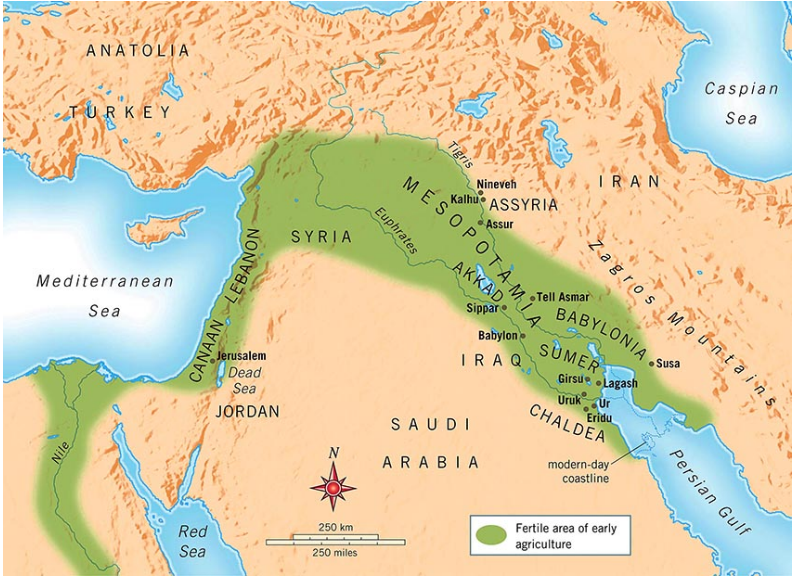
\includegraphics[width=.9\linewidth]{./img/fertileCrescent.png}
\caption{Fertile Crescent of early agriculture}
\end{figure}

\begin{itemize}
\item Framed in Today's Geopolitical Landscape
\end{itemize}
\begin{figure}[htb]
\centering
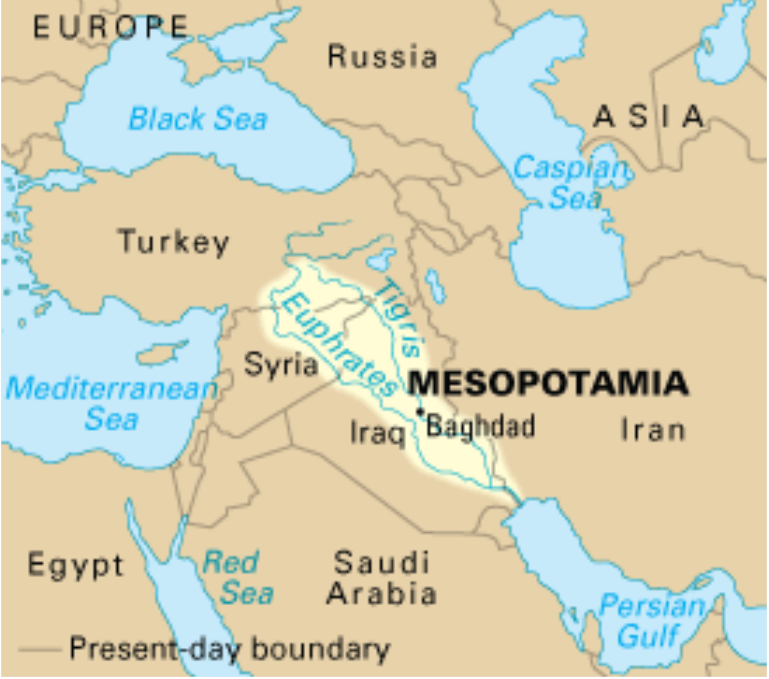
\includegraphics[width=.9\linewidth]{./img/GeoLand.png}
\caption{More modern representation of area.}
\end{figure}

\subsection{Home to diverse groups of people}
\label{sec-3-4}
\begin{itemize}
\item Sumerians

\item Akkadians

\item Persians

\item Babylonians

\item \textbf{Some of the oldest societies}
\end{itemize}

\subsection{Hummurabi and his Code}
\label{sec-3-5}
\begin{itemize}
\item If any one finds runaway male or female slaves in the open country and bring them to their masters, the master of the slaves shall pay him two shekels of silver.

\item If any one is commiting a robbery and is caught, then he shall be put to death.

\item If a tevern-keeper (feminine) does not accept corn according to gross weight in payment of a drink, but takes money, and the price of the drink is less than that of the corn, she shall be convicted and thrown into the water.

\item If a son strike his father, his hands be hewn off.

\item If a man knock out the teeth if his equal, his teeth shall be knocked out.

\item If a barber, without the knowldedge of his master, but the sign of a slave on a slave not to be sold, the hands of the barber shall be cut off.

\item If a slave says to his master: "You are not my master" - if they convict him his master shall cut off his ear.
\end{itemize}

\subsection{Timeline}
\label{sec-3-6}
\begin{itemize}
\item Goes back to 3500 BC

\item Civilization arose around present day Iraq

\item Communicated throught a written language: cuneiform
\end{itemize}
\begin{figure}[htb]
\centering
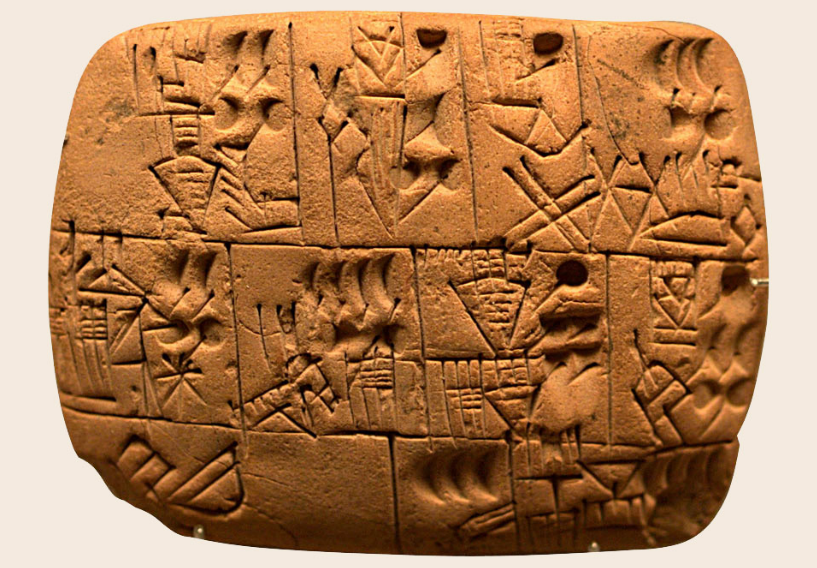
\includegraphics[width=.9\linewidth]{./img/CuneiformTablet.png}
\caption{Cuneiform tablet writing}
\end{figure}

\subsection{Literature: \emph{The Epic of Gilgamesh}}
\label{sec-3-7}
\begin{itemize}
\item Written around 2100 BC

\item About 12 books, or about 5 epic poems

\item \texttt{He saw the Scret, discovered the HIdden, he brought information of (the time) before the Flood. He went on a distance hourney, pushing himeelsf to exhaustion, but then was brought peace} (1.5-8)
\end{itemize}

\subsection{Technological Achievement}
\label{sec-3-8}
\begin{itemize}
\item Metalworking (Bronze, Copper, Gold, and eventually iron)

\item Glass making

\item Textile Weaving

\item Water Storage/control
\end{itemize}

\subsubsection{Walls of Babylon \emph{Part of \textbf{Seven Wonder}}}
\label{sec-3-8-1}
\begin{figure}[htb]
\centering
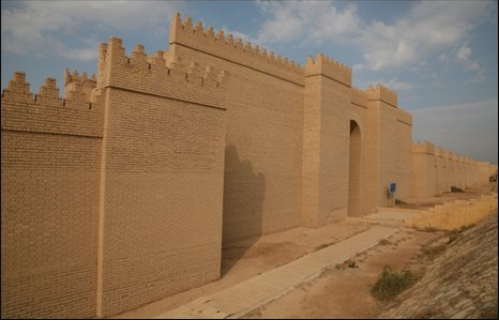
\includegraphics[width=.9\linewidth]{./img/WallsBabylon.png}
\caption{Wall of Babylon}
\end{figure}

Provides great security, allows for focus on other aspects of life.

\subsubsection{{\bfseries\sffamily TODO} Archimedes Screw: Verify location of possible garden's location with Driggers.}
\label{sec-3-8-2}
Some scholars believe that this was how the supposed \emph{handing gardens} were irrigated.
\begin{figure}[htb]
\centering
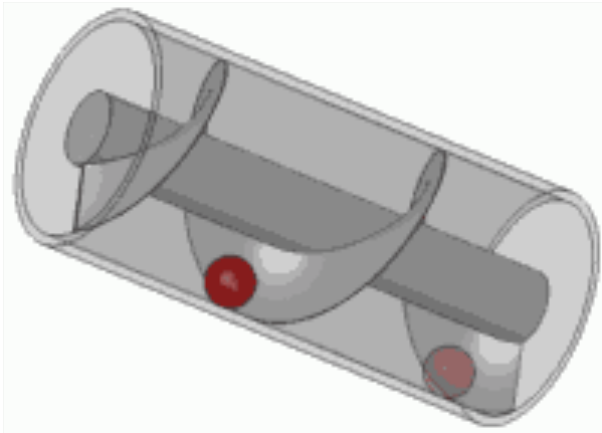
\includegraphics[width=.9\linewidth]{./img/archScrew.png}
\caption{Archimedes Screw}
\end{figure}

\begin{figure}[htb]
\centering
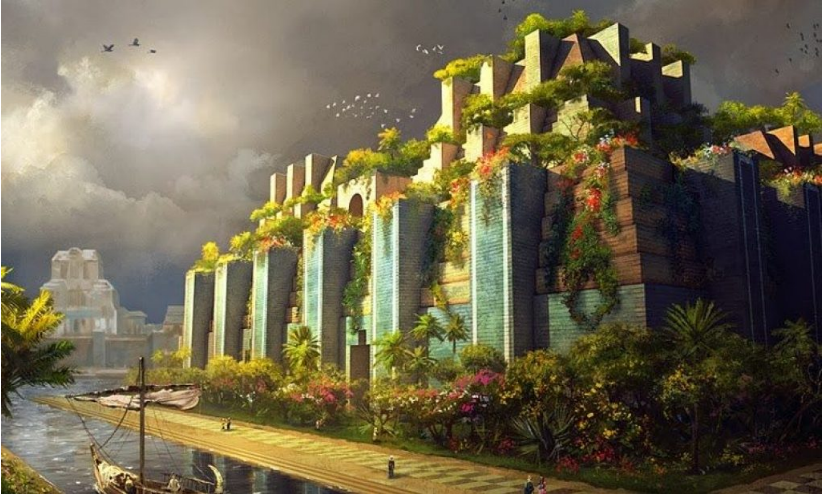
\includegraphics[width=.9\linewidth]{./img/HangingGardens.png}
\caption{Hanging Gardens}
\end{figure}

\begin{figure}[htb]
\centering
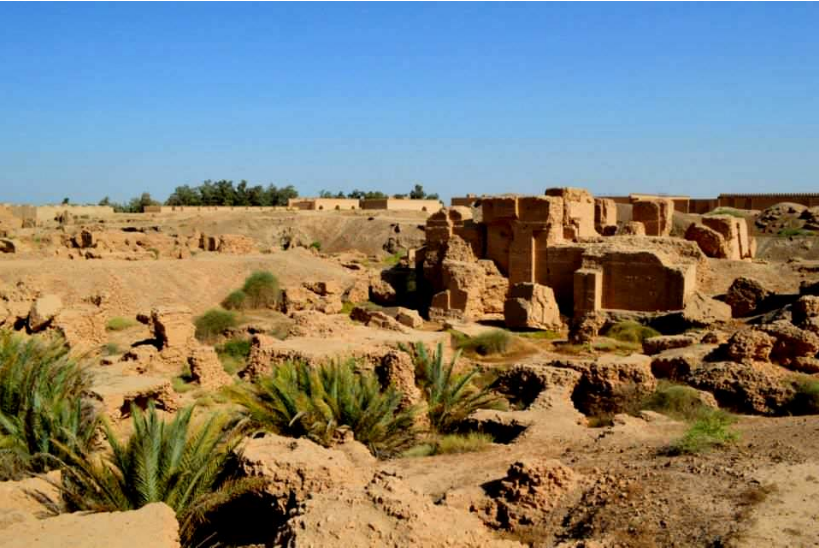
\includegraphics[width=.9\linewidth]{./img/HangingGardens2.png}
\caption{Possible location of gardens}
\end{figure}


\subsubsection{Assyrian Pottery}
\label{sec-3-8-3}
Allows travel to further distances away from immediate water access.

\subsubsection{Astronomy - Wrote down observations}
\label{sec-3-8-4}
This allows us to \emph{track} backwards in time and \emph{line up} our time line, and understandings with theirs.

\subsubsection{Mathematics}
\label{sec-3-8-5}
Mostly derived from needs of scribes, and clerks, doing tax calculations, record keeping was also important.

\begin{figure}[htb]
\centering
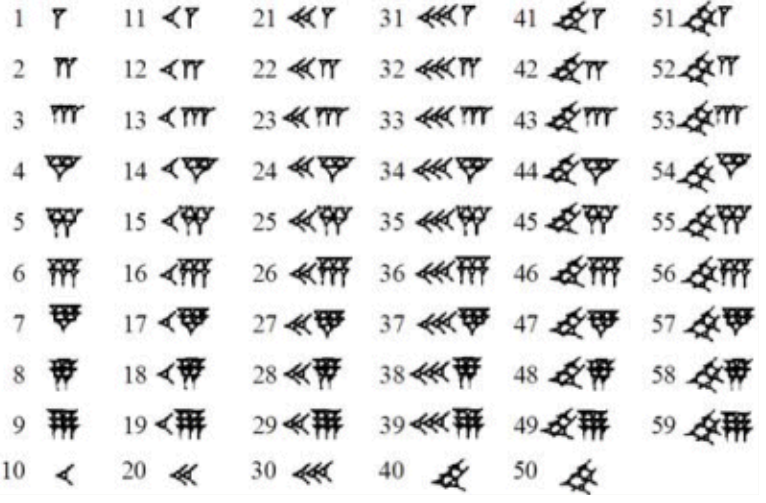
\includegraphics[width=.9\linewidth]{./img/CuneMath.png}
\caption{Cuneiform Mathematics symbols.}
\end{figure}

\begin{figure}[htb]
\centering
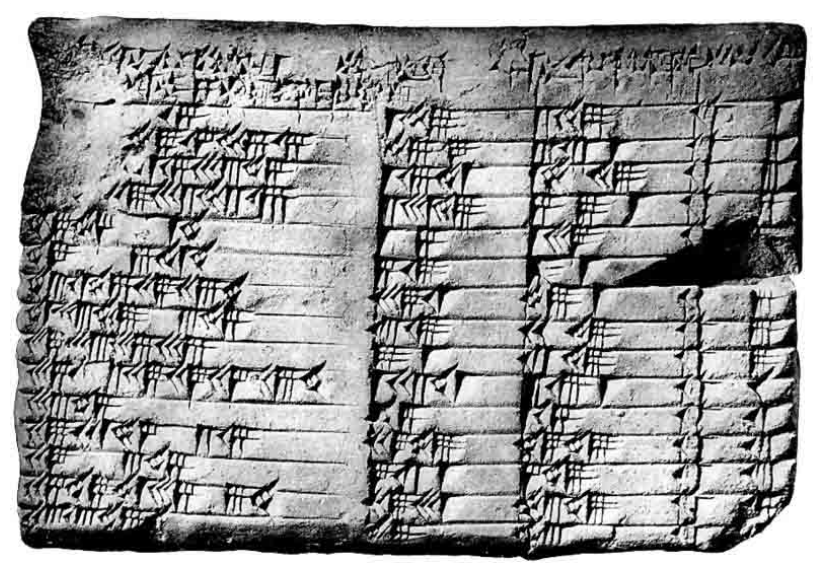
\includegraphics[width=.9\linewidth]{./img/acctRecs.png}
\caption{Accounting Records}
\end{figure}

\subsubsection{Medicine}
\label{sec-3-8-6}
\begin{figure}[htb]
\centering
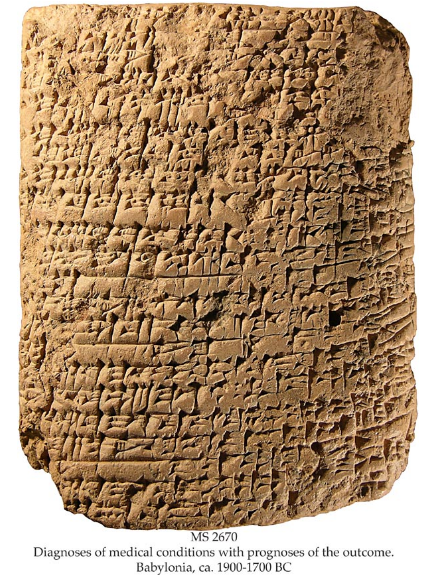
\includegraphics[width=.9\linewidth]{./img/MedRecs.png}
\caption{Medical Records}
\end{figure}

Scholars of early medicine started taking \emph{notes} about what methods worked, and those that didn't
% Emacs 25.3.1 (Org mode 8.2.10)
\end{document}
